\documentclass[a4paper,10pt]{article}
\usepackage{fontspec}
\usepackage{setspace}
\usepackage{booktabs}
\usepackage{amsmath}
\usepackage{cancel}
\usepackage{graphicx}
\usepackage{biblatex}
\usepackage{float}
\usepackage{tabularx}
\usepackage{booktabs}

\setmainfont{arial}
\setstretch{1.15}
\addbibresource{refs.bib}

\title{Deep learning and Optimization}
\author{Arif Suganda\\
        Tadulako University\\
        \texttt{f5522530002@untad.ac.id}
}

\begin{document}
\maketitle

\section{Neural Network}

Neural networks are computational models inspired by the human brain, consisting of interconnected nodes (neurons) that process information. 
Each neuron receives inputs, applies weights to them, adds a bias, and then passes the result through an activation function to produce an output.
Neural networks is calculated using the following steps:

\subsection{Forward propagation}
Forward propagation is used to predict the output of the neural network, these processes divided into several steps, which are:

\noindent
Sum of weighted inputs and bias, which is calculated as follows:
\begin{equation}\label{eq:sum_weight_bias}
    z = \sum_{i=1}^{n} w_i x_i + b
\end{equation}

Activation function, using sigmoid activation function, which is defined as:
\begin{equation}\label{eq:sigmoid}
    \sigma(z) = \frac{1}{1 + e^{-z}}
\end{equation}

Using the output we can interpret the output as a probability of binary class and can be converted to binary output using a threshold.
The threshold can be interpreted as follows:
\begin{equation}\label{eq:threshold}
    \hat{y} = \begin{cases}
        1 & \text{if } \sigma(z) \ge 0.5 \\
        0 & \text{if } \sigma(z) < 0.5
    \end{cases}
\end{equation}

\subsection{Backpropagation}
Backpropagation is used to calculate the gradient which is the rate of error weights and biases contibuted from the calculation of the loss function.
These processes divided into several steps, which are:

Calculate the loss function, for this example using Binary Cross-Entropy (BCE), which is defined as:
\begin{equation}\label{eq:bce_loss}
    L = -\left[ y \log(\hat{y}) + (1 - y) \log(1 - \hat{y}) \right]
\end{equation}

Calculate the derivative of the loss function ($L$) with respect to the sum of weighted inputs and bias (z) is calculated using the chain rule of calculus:
\begin{align}\label{eq:chain_rule}
\intertext{Chain rule application}
    \frac{\partial L}{\partial z} &= \frac{\partial L}{\partial \hat{y}} \cdot \frac{\partial \hat{y}}{\partial z} \\
\intertext{Derivative of Loss with respect to Prediction}
    \frac{\partial L}{\partial \hat{y}} &= -\left[ \frac{y}{\hat{y}} - \frac{1-y}{1-\hat{y}} \right] = \frac{\hat{y} - y}{\hat{y}(1-\hat{y})} \\
\intertext{Derivative of Prediction with respect to Sum of Weighted Inputs and Bias}
    \frac{\partial \hat{y}}{\partial z} &= \hat{y}(1 - \hat{y}) \\
\intertext{Combined Delta Calculation}
    \frac{\partial L}{\partial z} &= \frac{\hat{y} - y}{\cancel{\hat{y}(1-\hat{y})}} \cdot \cancel{\hat{y}(1 - \hat{y})} \nonumber \\
    \frac{\partial L}{\partial z} &= \hat{y} - y
\end{align}

\noindent
Update the weights and bias, we use the following formulas:
\begin{align}\label{eq:update_weights_bias}
    w_i &\leftarrow w_i - \alpha \cdot \frac{\partial L}{\partial w_i} \\
    b &\leftarrow b - \alpha \cdot \frac{\partial L}{\partial b}
\end{align}

\subsection{Analysis}
The core of the backpropagation, which is used to update weights and biases of each neuron, relies chain rule of derivative in mathematics.
The chain rule is used to calculate the gradient of each weights and biases, which is the rate of contribution of each weight or biase to produce the loss function value.

By knowing the gradient, each weight and bias can be change to minimize the loss function.
In multi-dimensional function the gradient is a vector represent the ``slope'' which can be ``lead'' into its lowest posible value.
The ``lead'' process to reduce loss function is the core of the learning process of neural network.

\section{Impelementation}

The implementation consist of:
\begin{enumerate}
    \item Dataset of backpropagation will use MNIST dataset~\cite{lecun2010mnist}, which is a hand written image dataset.
    \item The network architecture used is convolutional neural network (CNN)
    \item The netowrk consist of an input layer, 3 hidden layer and an output layer.
    \item The architecture can be seen in Figure~\ref*{fig:architecture}
\end{enumerate}

\begin{figure}[H]
    \centering
    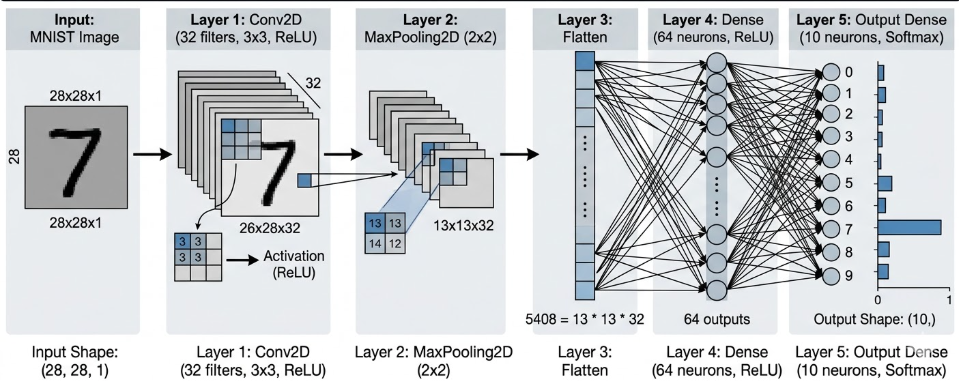
\includegraphics[width=1\textwidth]{architecture.png} 
    \caption{Network Architecture}\label{fig:architecture}
\end{figure}

The codes for this implementation are:
\begin{verbatim}
import tensorflow as tf
from tensorflow.keras import layers, models
import matplotlib.pyplot as plt

# Load and Preprocess Dataset
mnist = tf.keras.datasets.mnist
(x_train, y_train), (x_test, y_test) = mnist.load_data()

x_train = x_train.reshape((
    60000, 28, 28, 1)).astype('float32') / 255
x_test = x_test.reshape((
    10000, 28, 28, 1)).astype('float32') / 255

# Build and Compile Model
model = models.Sequential([
    layers.Conv2D(32, (3, 3), activation='relu', 
    input_shape=(28, 28, 1)),
    layers.MaxPooling2D((2, 2)),
    layers.Flatten(),
    layers.Dense(64, activation='relu'),
    layers.Dense(10, activation='softmax')
])

model.compile(optimizer='adam',
              loss='sparse_categorical_crossentropy',
              metrics=['accuracy'])

# Training
print("Starting training...")
history = model.fit(
    x_train, y_train, 
    epochs=10, 
    batch_size=64,
    validation_split=0.2,
    verbose=1
)

# Visualize

fig, (ax1, ax2) = plt.subplots(1, 2, figsize=(14, 5))

# Loss function
ax1.plot(history.history['loss'], 
label='Training Loss', color='blue', lw=2)
ax1.plot(history.history['val_loss'], 
label='Validation Loss', color='red', linestyle='--', lw=2)
ax1.set_title('Training and Validation Loss', fontsize=14)
ax1.set_xlabel('Epochs', fontsize=12)
ax1.set_ylabel('Loss (Error)', fontsize=12)
ax1.legend()
ax1.grid(True)

# Accuracy
ax1_acc = ax2 
ax1_acc.plot(history.history['accuracy'], 
label='Training Accuracy', color='blue', lw=2)
ax1_acc.plot(history.history['val_accuracy'], 
label='Validation Accuracy', color='red', linestyle='--', lw=2)
ax1_acc.set_title('Training and Validation Accuracy', 
fontsize=14)
ax1_acc.set_xlabel('Epochs', fontsize=12)
ax1_acc.set_ylabel('Accuracy', fontsize=12)
ax1_acc.legend()
ax1_acc.grid(True)

# Display
plt.tight_layout
\end{verbatim}

The results can be seen in Figure~\ref*{fig:loss_and_accuracy}

\begin{figure}[H]
    \centering
    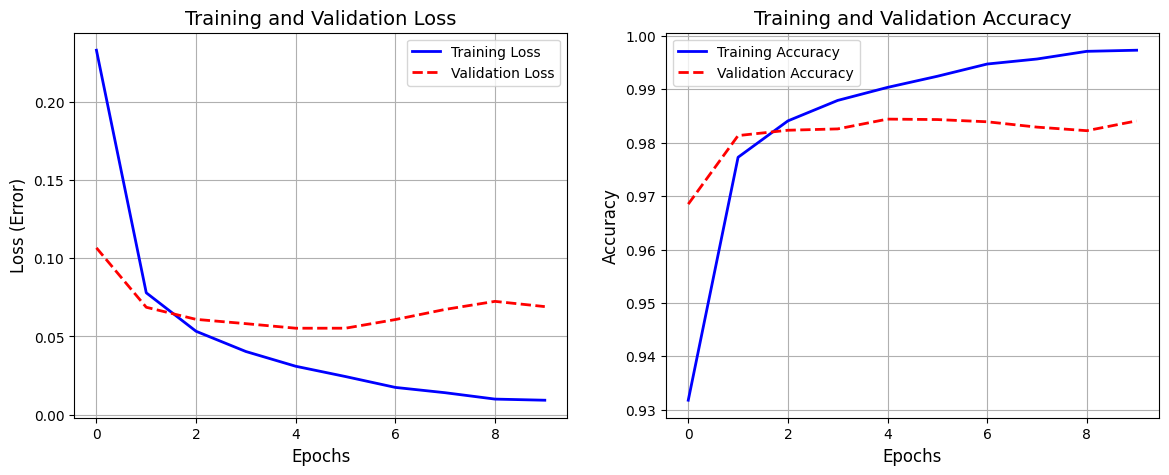
\includegraphics[width=1\textwidth]{loss_and_accuracy.png} 
    \caption{Loss and accuracy}\label{fig:loss_and_accuracy}
\end{figure}

\section{Optimization}
In deep learning training optimization is used to speed up learning process.

\subsection{Adaptive Moment Estimation (Adam)}
Code:
\begin{verbatim}
model.compile(
    optimizer='adam',
    loss='sparse_categorical_crossentropy',
    metrics=['accuracy'])
\end{verbatim}

Result can be seen in Figure~\ref*{fig:loss_and_accuracy}

\subsection{Stochastic Gradient Descent (SGD)}

Code:
\begin{verbatim}
from tensorflow.keras import layers, models, optimizers

custom_sgd = optimizers.SGD(learning_rate=0.01, momentum=0.9)

model.compile(optimizer=custom_sgd,
              loss='sparse_categorical_crossentropy',
              metrics=['accuracy'])
\end{verbatim}

Result can be seen in ~\ref*{fig:sgd}
\begin{figure}[H]
    \centering
    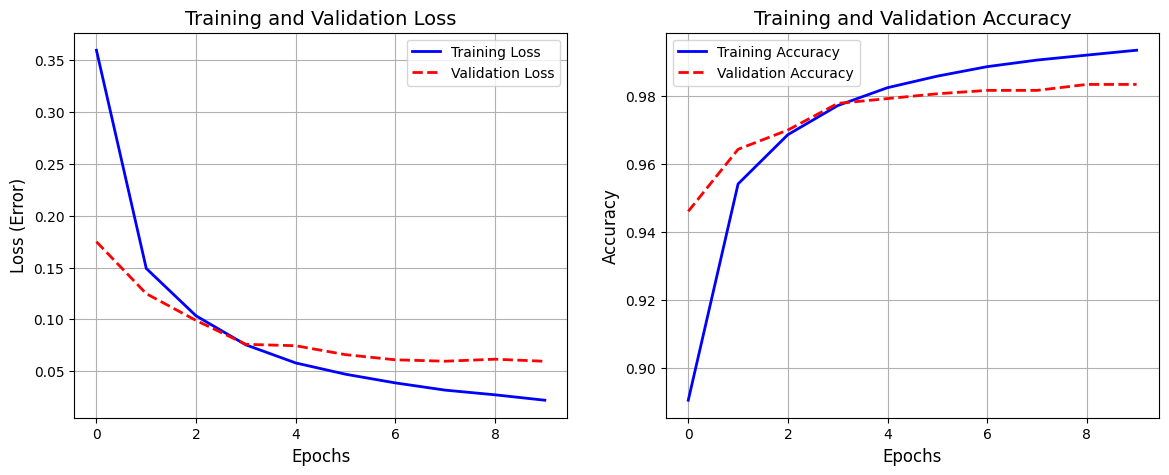
\includegraphics[width=1\textwidth]{sgd.png} 
    \caption{Stochastic gradiet descent}\label{fig:sgd}
\end{figure}

\subsection{Analysis}
As we can see in the Figure~\ref*{fig:loss_and_accuracy} and Figure~\ref*{fig:sgd} 
in the begining the loss function changes in adam is faster than in SGD, and SGD change is over all more stable than adam.
The loss function in adam is lower \textbf{0.0079} compared to \textbf{0.0231} in SGD.
Overall the reduction of loss function in adam is faster compared to SGD while the stablity of changes is better in SGD.

\section{Regularization}

Regularization is a method to prevent the network from overfitting.

\subsection{Dropout}

Code:
\begin{verbatim}
model = models.Sequential([
    layers.Conv2D(32, (3, 3), 
    activation='relu', input_shape=(28, 28, 1)),
    layers.MaxPooling2D((2, 2)),
    layers.Flatten(),
    layers.Dropout(0.5),
    layers.Dense(64, activation='relu'),
    layers.Dense(10, activation='softmax')
])
\end{verbatim}

Result:
\begin{figure}[H]
    \centering
    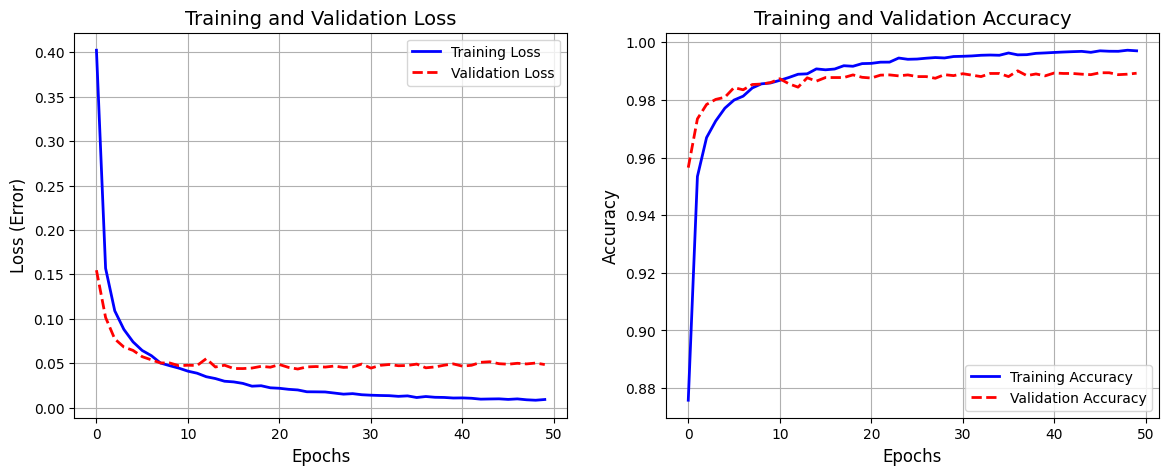
\includegraphics[width=1\textwidth]{dropout.png} 
    \caption{Dropout}\label{fig:dropout}
\end{figure}
\section{Analysis}
Shown in Figure~\ref*{fig:dropout} the stability in loss function and accuracy of validation dataset is slower than in Figure~\ref*{fig:loss_and_accuracy}.
But it also shown that it is more stable than in the previous implementation, 
although the loss function and accuracy in training dataset is slowly getting lower,
the loss function and accuracy in validation dataset is quite stable.
This show that the dropout regulation works perfectly and dont follow the trend in training dataset.

\printbibliography{}

\end{document}